\documentclass[11pt]{report}

\usepackage{amsmath,braket,mathtools}
%\usepackage{showframe}

\newcommand{\C}{a^{\dagger}}
\newcommand{\D}{a}

\newcommand{\Mv}{\vec{\gamma}}
\newcommand{\Mx}{\gamma^x}
\newcommand{\My}{\gamma^y}

\newcommand{\en}{\varepsilon}
\newcommand{\eff}{_{\textnormal{eff}}}

\begin{document}

\title{Level crossings in the Floquet quasienergies of the Kitaev chain}
\maketitle

\subsection*{The Model}

We consider the Kitaev chain model\cite{Kitaev2001} with periodic driving of the on-site potential\cite{Dutta2013},
%
\begin{equation}
	H(t) = \sum_{n=1}^{N-1}( t\C_{n}\D_{n+1} + \Delta\C_{n}\C_{n+1} + \textrm{H.c.}) + \mu(t)\sum_{n=1}^{N} 2(\C_{n}\D_{n} - 1),
\end{equation}
%
where
%
\begin{equation}
	\mu(t) = \mu_0 + \mu_1 T \sum^{\infty}_{\mathclap{n=-\infty}} \delta(t-nT).
\end{equation}
%
We may write the Hamiltonian in terms of $2N$ Majorana fermions defined at each site $n$ as
$
\Mx_n \equiv \D_n+\C_n,
\My_n \equiv i(\D_n - \C_n).
$
After the transformation, the Hamiltonian becomes
$
H(t) = (i/4)\Mv^{\dagger} M(t) \Mv,
$
where
$
\Mv^{\dagger} \equiv [\Mx_1, \My_1, \Mx_2, \My_2 \dots],
$
and
%
\begin{equation}
		M[\mu(t),J_x,J_y] = \left(\begin{matrix}
		0 & \mu(t) & 0 & -J_y \\
		-\mu(t) & 0 & J_x & 0 & \dots \\
		0 & -J_x & 0 & \mu(t) \\
		J_y & 0 & -\mu(t) & 0\\
		 & & \vdots & 
	\end{matrix} \right)
\end{equation}	
%
with
$
J_x \equiv (\gamma-\Delta)/2, J_y \equiv (\gamma+\Delta)/2.
$
In the Heisenberg picture, the time evolution of the Majorana operators is given by


the time-ordered operator 
%
\begin{equation}
	U(T) = \mathcal{T} \left[e^{ \int^T_0 M(t)dt}\right],
\end{equation}
%
as shown in \cite{Dutta2013}. Since the potential driving occurs right at the limits of the integral, it would make sense to consider a symmetric evolution operator as in \cite{Dutta2013}, but we choose a simpler 2-term operator which is equivalent in terms of the quasienergies:
%
\begin{equation}
U(T) = e^{M_1 T}e^{M_0 T} = e^{-iH_{F}T}
\end{equation}
%
where $M_0 = M[\mu_0,J_x,J_y]$, $M_1 = M[\mu_1,0,0]$ and where we define an effective Hamiltonian $H_{F}$ which can be obtained as an expansion using the BCH formula, giving
%
\begin{equation}
-iH_{F} = M_0 + M_1 + \frac{T}{2}[M_0,M_1] +\frac{T^2}{12}([M_0,[M_0,M_1]]+[M_1,[M_1,M_0]])+\cdots
\end{equation}
%
In zero order in $T$ the system behaves as a static Kitaev chain with potential $\mu = \mu_0 + \mu_1$. Calculating explicitly the next term, we obtain 
%
\begin{equation}
\label{eq:1st_order}
[M_0,M_1] = \Delta\mu_1 \left(\begin{matrix}
		0 & 0 & -1 & 0 \\
		0 & 0 & 0 & 1 & \dots \\
		1 & 0 & 0 & 0 \\
		0 & -1 & 0 & 0\\
		 & & \vdots & 
	\end{matrix} \right),
\end{equation}
%
so for small $\mu_1$ and $\Delta$ we also expect an approximation to a static Kitaev chain to be valid. The quasienergies $\en$ are the eigenvalues of $H_F$, however, energies of $\en$ or $\en+2\pi n/T$ are equivalent in terms of the time evolution over a period, so we will only consider quasienergies in the first Time Brillouin zone: $ -\pi/T \leq \en < \pi/T$. Also, $M_1$ is simple enough ($2\times2$ block-diagonal) that we can calculate $e^{M_1 T}$ explicitly:
%
\begin{equation}
	e^{M_1 T} = \left(\begin{matrix}
			\cos(\mu_1 T) & \sin(\mu_1 T) & 0 & 0 \\
			-\sin(\mu_1 T) & \cos(\mu_1 T) & 0 & 0 & \dots \\
			0 & 0 & \cos(\mu_1 T) & \sin(\mu_1 T) \\
			0 & 0 & -\sin(\mu_1 T) & \cos(\mu_1 T)\\
			  & & \vdots & 
	\end{matrix} \right),
\end{equation}
% 
and we see that we can also restrict $\mu_1$ to a Brillouin zone: $ 0 \leq \mu_1 < 2\pi/T$. We also have that
%
\begin{equation}
e^{M[\mu_1 +\pi/T]T} = e^{M[\mu_1]T+M[\pi/T]T} = e^{M[\mu_1 T]}e^{M[\pi]}, 
\end{equation}
where all other parameters of $M$ are zero, and from Eq. 7 we have $e^{M[\pi]} = -I = e^{i\pi I}$. Then,
%
\begin{equation}
e^{-iH_F[\mu_1+\pi/T]T} = e^{M[\mu_1]T}e^{M_0 T}e^{i\pi I} = e^{-i(H_F[\mu_1]-\pi/T)T}
\end{equation}
% 
I find this useful to understand the origin of the $\pi/T$ quasienergies. For small perturbing parameters we have seen that we can approximate the quasienergies by the energies of the static Kitaev chain, which has a well-known zero eigenvalue for $|\mu| < |\gamma|$, meaning we expect a $\pi/T$ eigenvalue for $|\mu-\pi/T| < |\gamma|$. 

\subsection*{Level crossings induced by $\mu_1$}

\begin{figure}
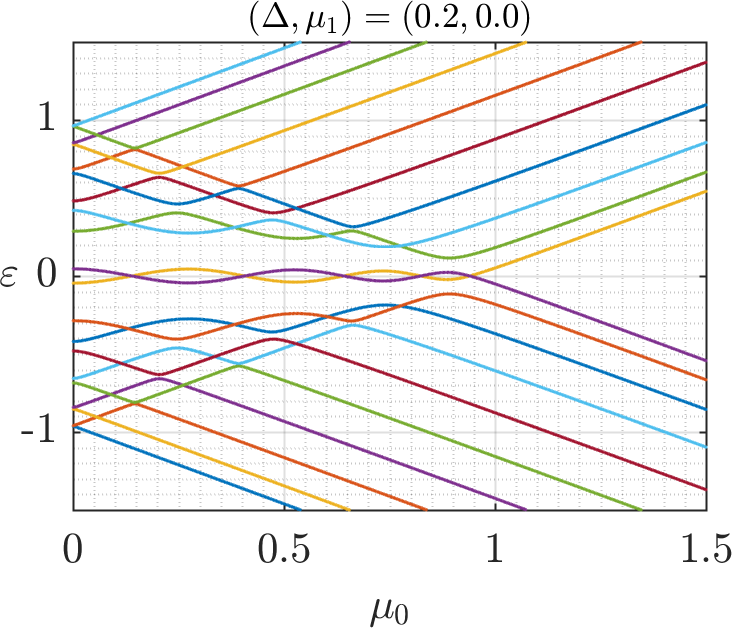
\includegraphics[width=0.5\textwidth]{Figures/Fig1.png}%
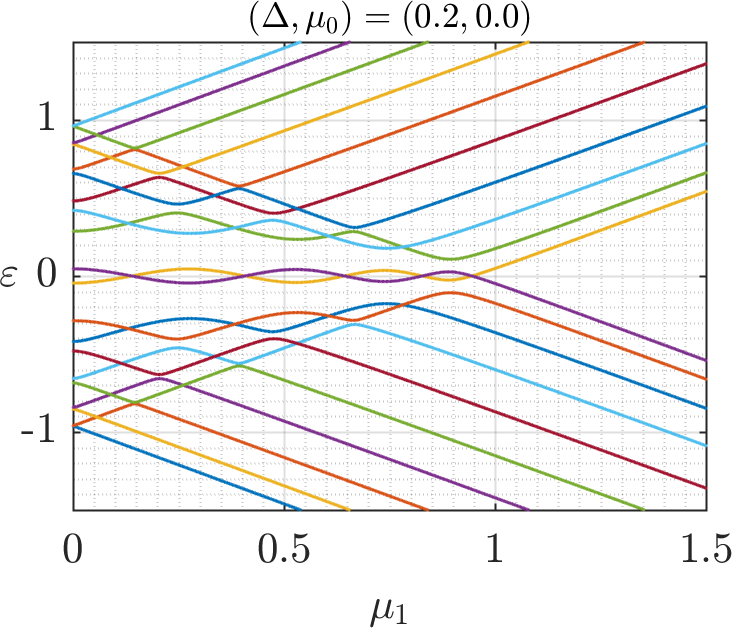
\includegraphics[width=0.5\textwidth]{Figures/Fig2.png}
\caption{Quasienergies for $N=10$, $T=1$ and $\Delta = 0.2$ as a function of $\mu_0$ (left) and $\mu_1$ (right).}
\label{Fig:1}
\end{figure}

For a finite size, the (close to) zero eigenvalues of the static Kitaev chain have oscillations when $\gamma^2 > \Delta^2$, causing $N$ crossings and consequently $N$ exact values of the potential in which there is an exact zero eigenvalue\cite{Gregoire2017,Ivo2017}. In Fig.~1 on the left, we show the quasienergies as a function of $\mu_0$, for $\mu_1 = 0$. Effectively, since for the chosen parameters the eigenvalues of $H_F$ are already contained in the first Brillouin zone, this is the spectrum of the static Kitaev chain. If we increase $T$ so that the quasienergies start to cross $\pm \pi/T$, the spectrum can become quite messy and thus more distant to the static spectrum, so we shall use $\gamma = 1$ and $T = 1$ always. I also don't think the system size is a big factor when studying the crossings. Increasing the system size will mainly increase the number of crossings and reduce exponentially the (close to) zero quasienergies, so we set $N = 10$ to further increase readability. We are left with $\Delta$, $\mu_{0,1}$ as our parameters. All further plots have $\mu_1$ on the $x$-axis. In Fig.~1 on the right, we confirm that we recover the static behaviour for small $\Delta$ and $\mu$.

\begin{figure}
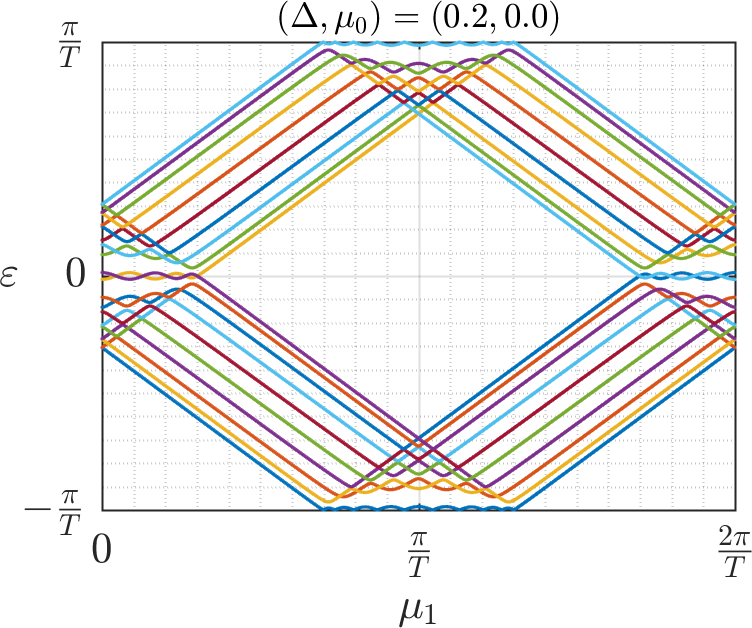
\includegraphics[width=0.5\textwidth]{Figures/Fig3.png}%
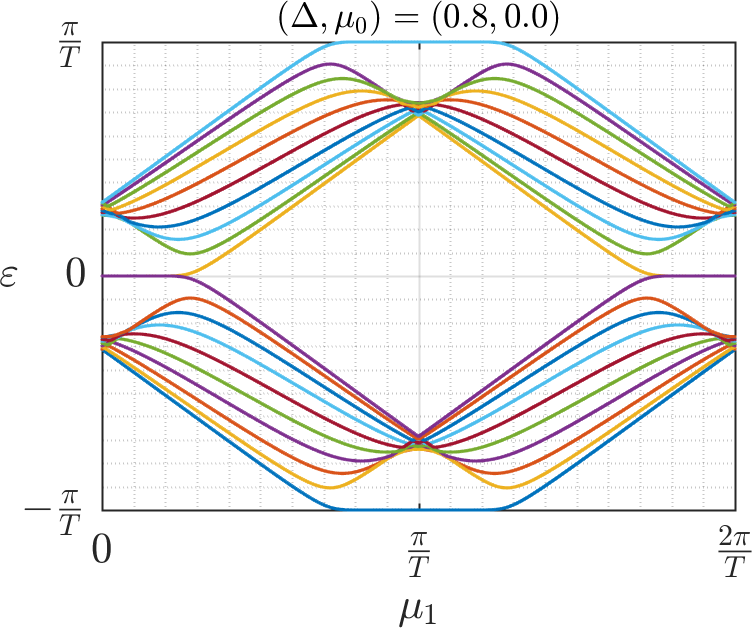
\includegraphics[width=0.5\textwidth]{Figures/Fig4.png}\\
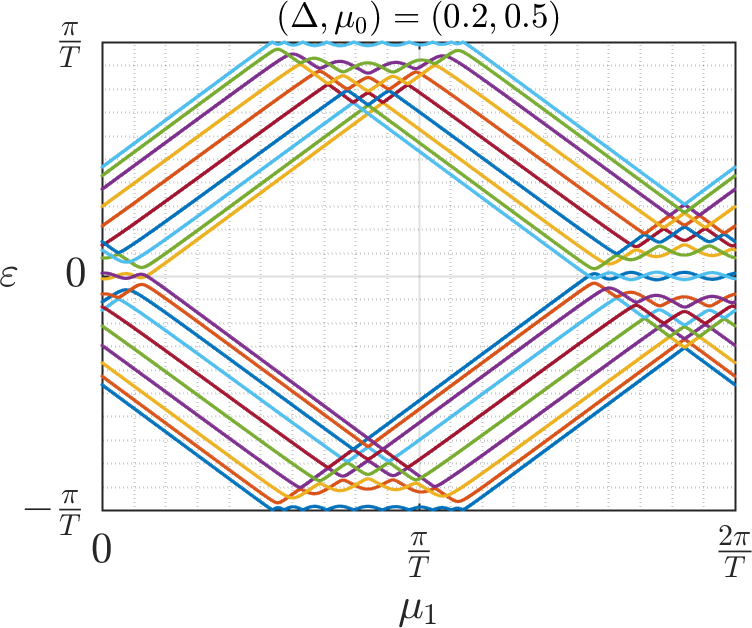
\includegraphics[width=0.5\textwidth]{Figures/Fig5.png}%
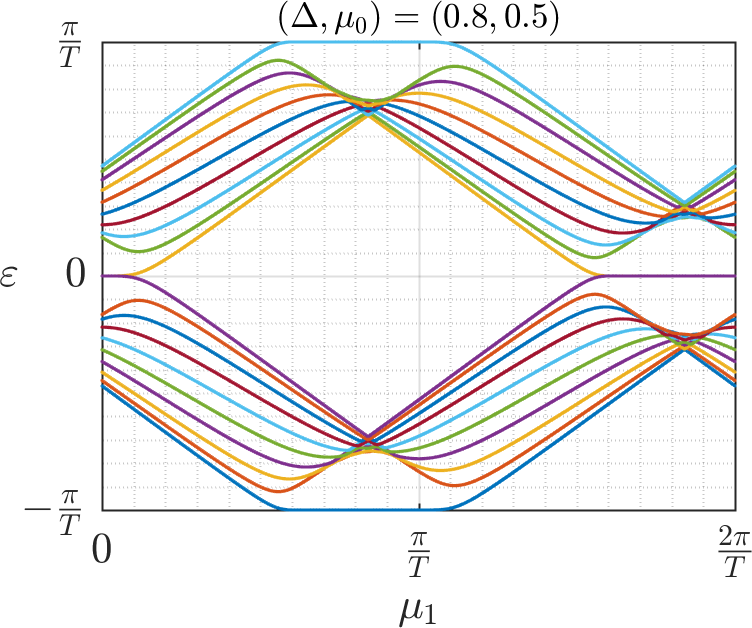
\includegraphics[width=0.5\textwidth]{Figures/Fig6.png}\\
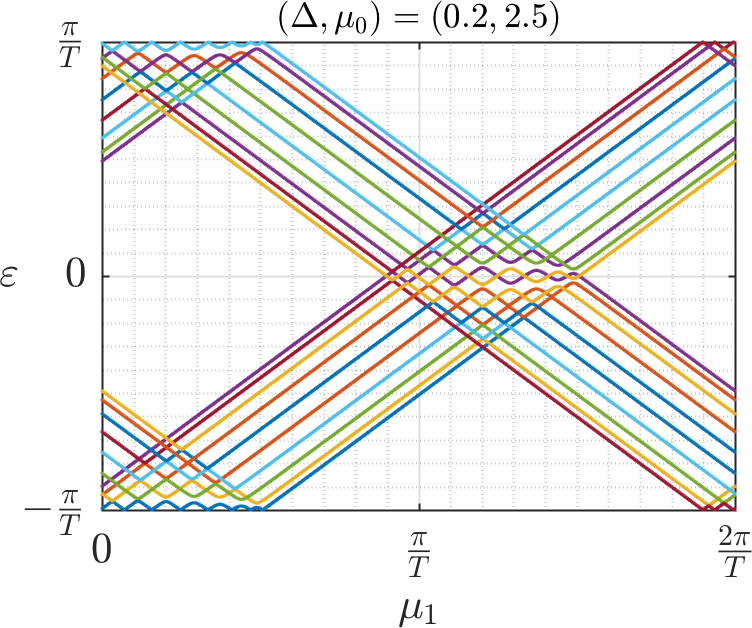
\includegraphics[width=0.5\textwidth]{Figures/Fig7.png}%
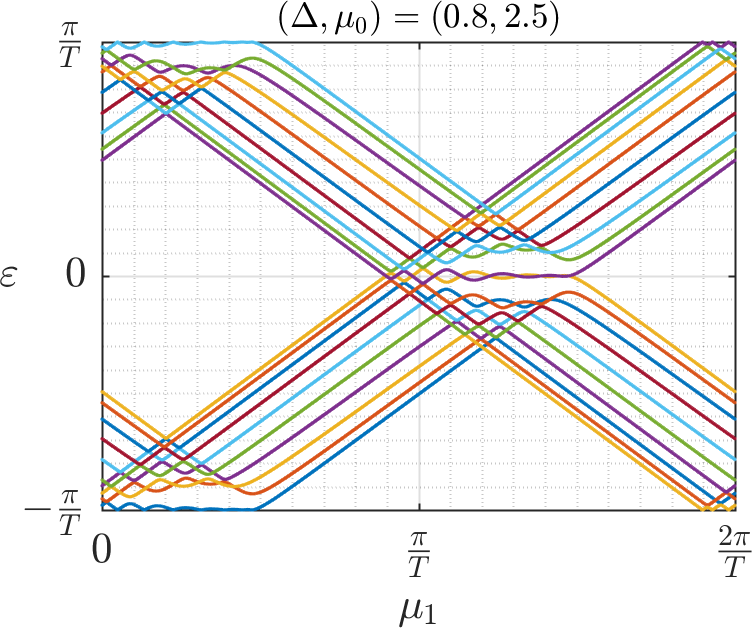
\includegraphics[width=0.5\textwidth]{Figures/Fig8.png}%
\caption{Quasienergies as a function of $\mu_1$ for small $\Delta$ (left) and large (right) and no static potential (top), low (middle) and high (bottom).}
\label{Fig:2}
\end{figure}

In Fig.~2 we have quasienergies for several $\Delta$ and $\mu_0$. In all of them we verify the presence of the $\pi/t$ quasienergy in the expected symmetric position. The energy oscillations are greater for small $\Delta$, which matches with the static model where all oscillations disappear in the limit $\Delta \rightarrow \gamma = 1$ (Transverse field Ising model). The main effect of $\mu_0$ is a translation, showing that $\mu = \mu_0 + \mu_1$ is the main parameter to consider. However, the effect on the crossings is worth of note. As seen more clearly in the right column, $\mu_0$ increases the oscillation amplitude asymmetrically. More than that, the oscillations even show up for $\Delta = 1$, as seen in Fig.~3, which means the driving can cause the same kind of level oscillations as in the static case even when the static Hamiltonian $M_0$ has no oscillations. The number of crossings of the zero quasienergies seems to be $N$, like the static case.

\begin{figure}
\centering
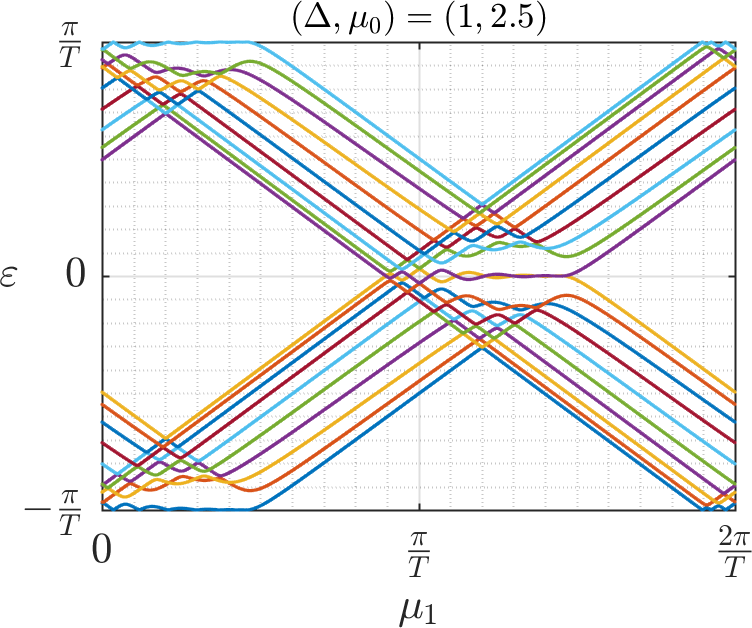
\includegraphics[width=0.5\textwidth]{Figures/Fig9.png}
\caption{Quasienergies as a function of $\mu_1$ for $\Delta = 1$.}
\label{Fig:3}
\end{figure}

\subsection*{Asymmetric effects due to $\mu_0$}
\begin{figure}
\centering
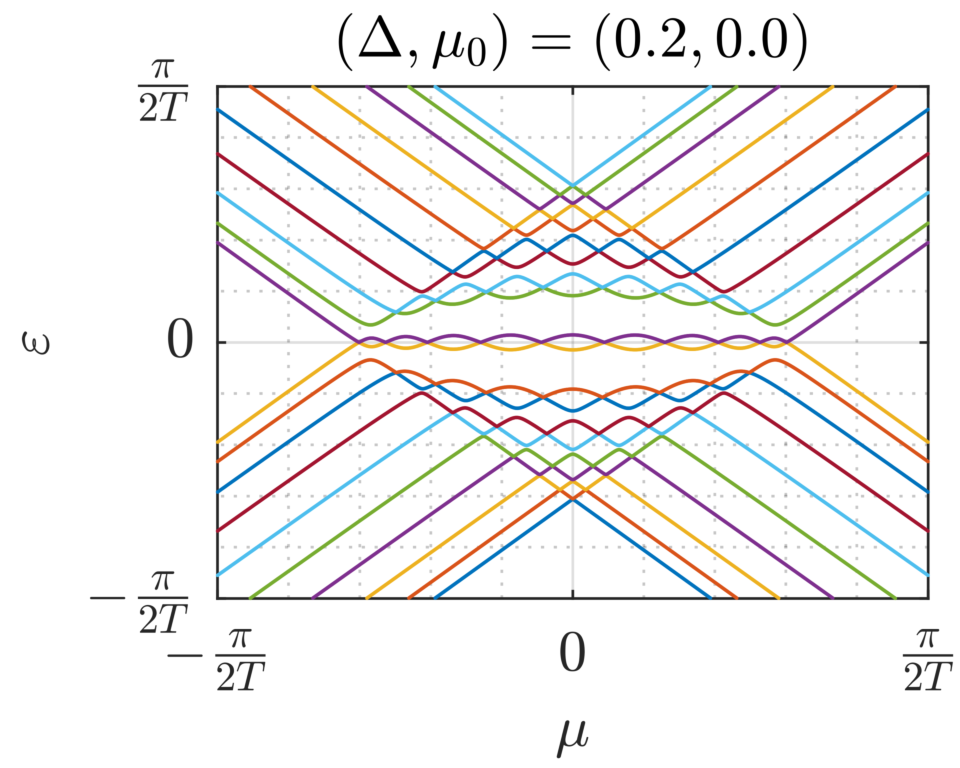
\includegraphics[scale=1]{Figures/New/Quasienergies_Exact1.png}%
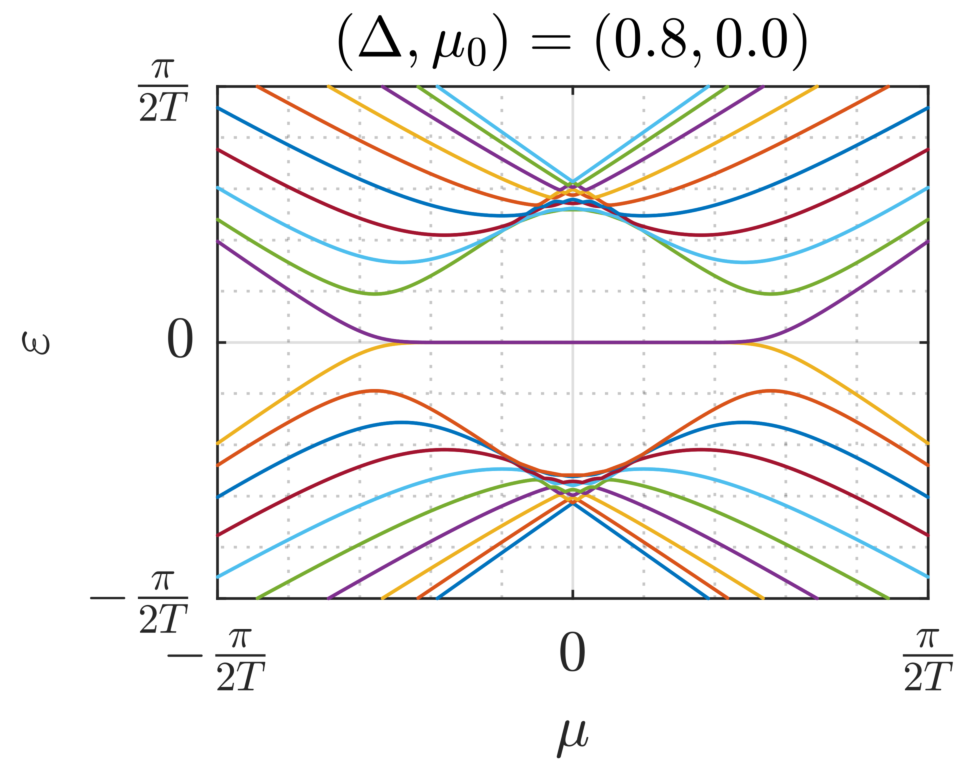
\includegraphics[scale=1]{Figures/New/Quasienergies_Exact2.png}\\
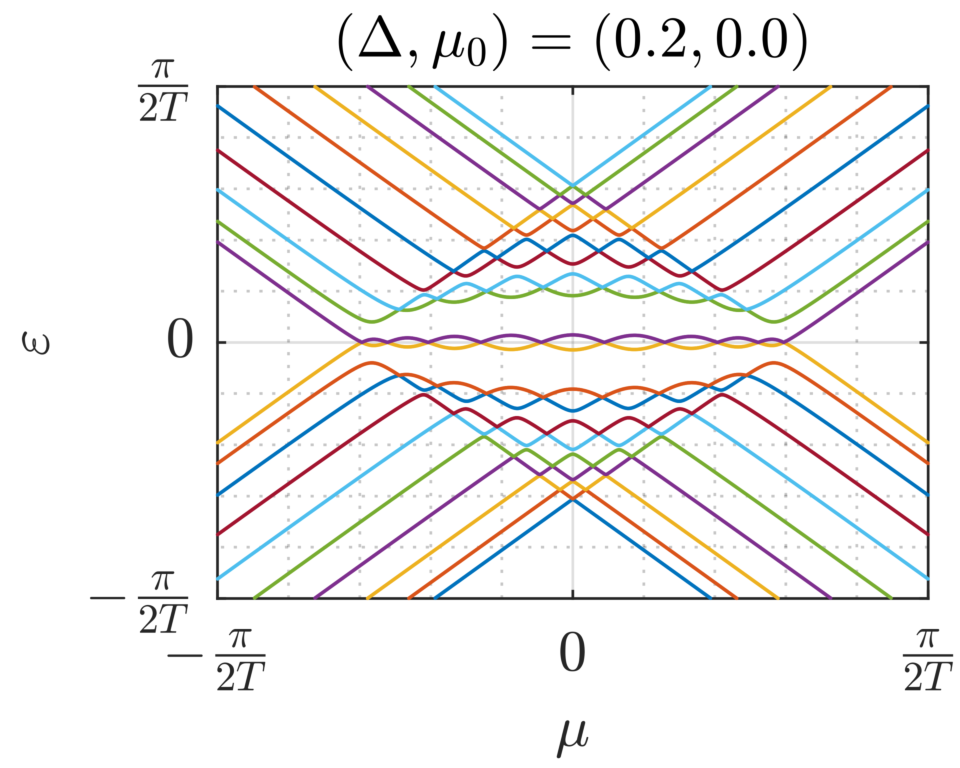
\includegraphics[scale=1]{Figures/New/Quasienergies_Expansion1.png}%
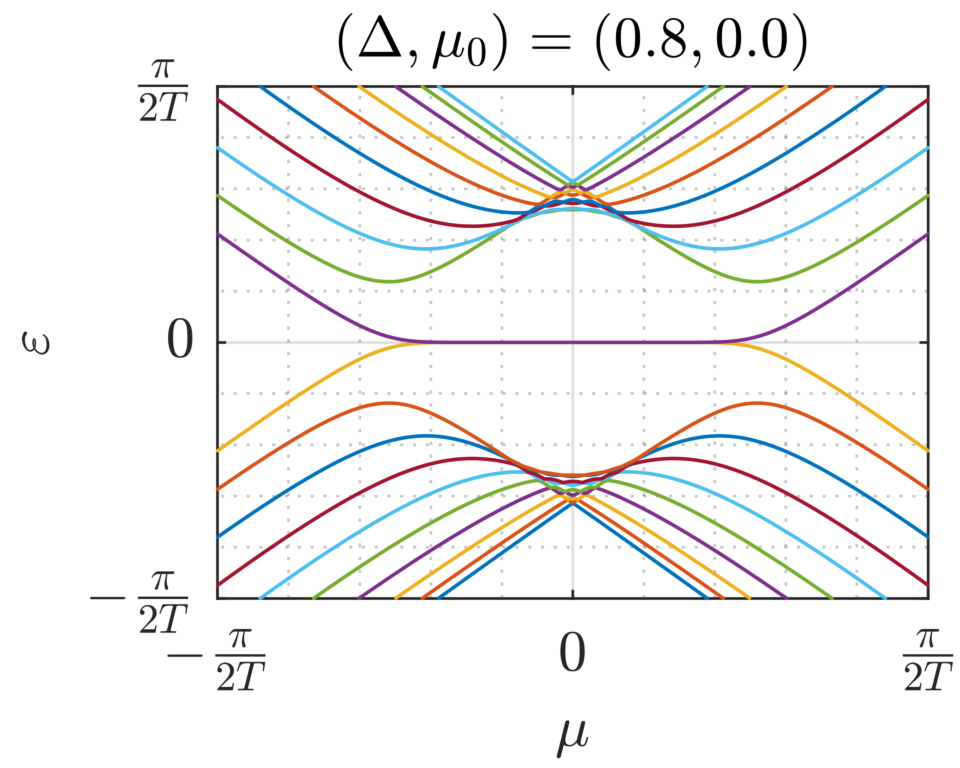
\includegraphics[scale=1]{Figures/New/Quasienergies_Expansion2.png}\\
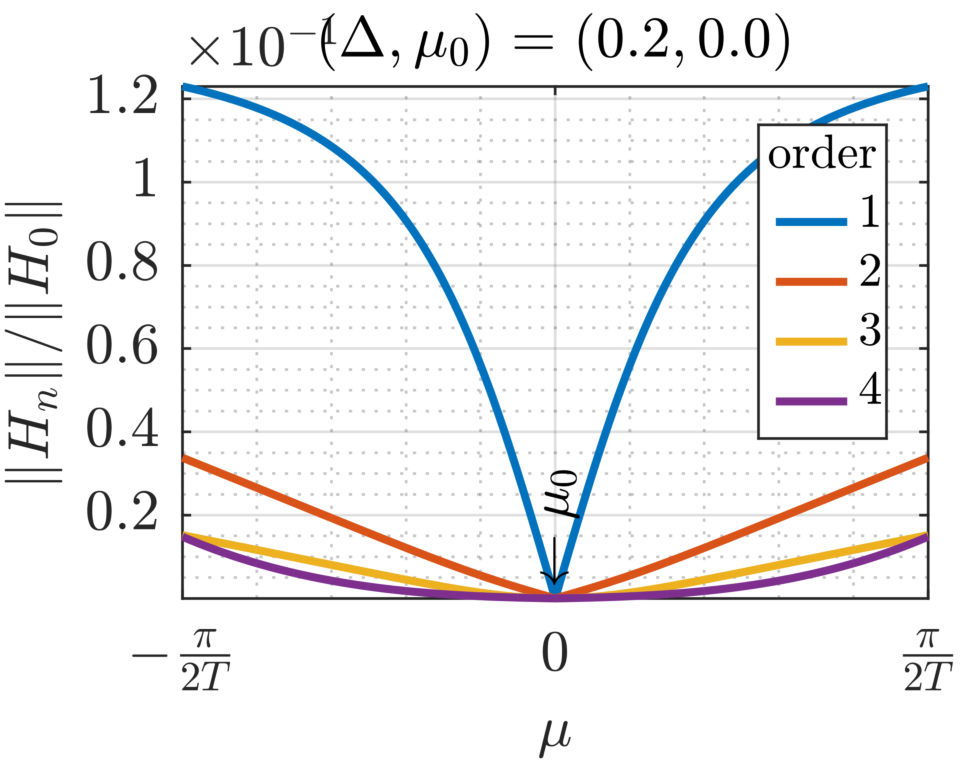
\includegraphics[scale=1]{Figures/New/Expansion_Amplitude1.png}%
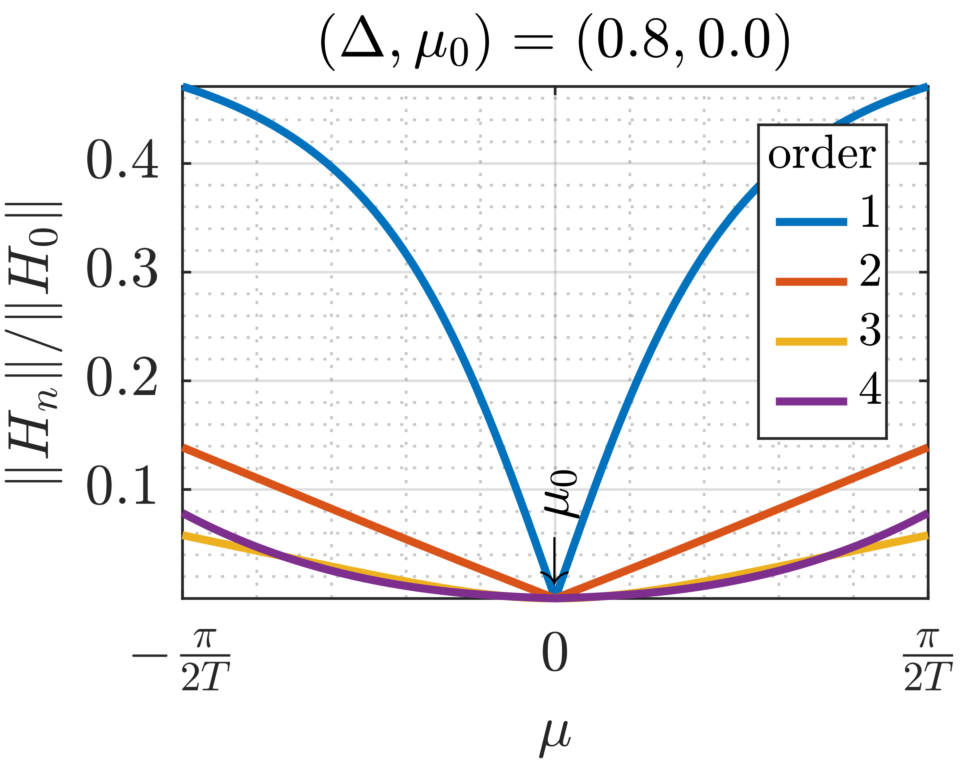
\includegraphics[scale=1]{Figures/New/Expansion_Amplitude2.png}\\
\caption{Top row: exact quasienergies. Middle row: quasienergies calculated by $2^{\text{nd}}$ order BCH approximation. Bottom row: relative norm of the four first BCH expansion terms.}
\label{Fig:4}
\end{figure}

\begin{figure}
\centering
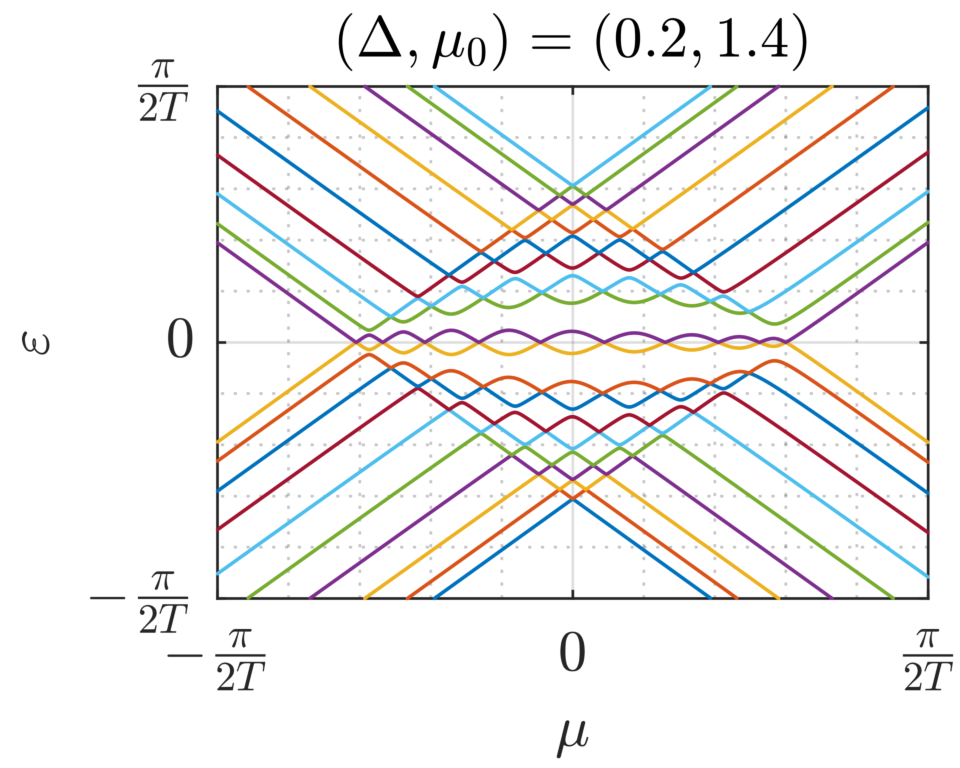
\includegraphics[scale=1]{Figures/New/Quasienergies_Exact3.png}%
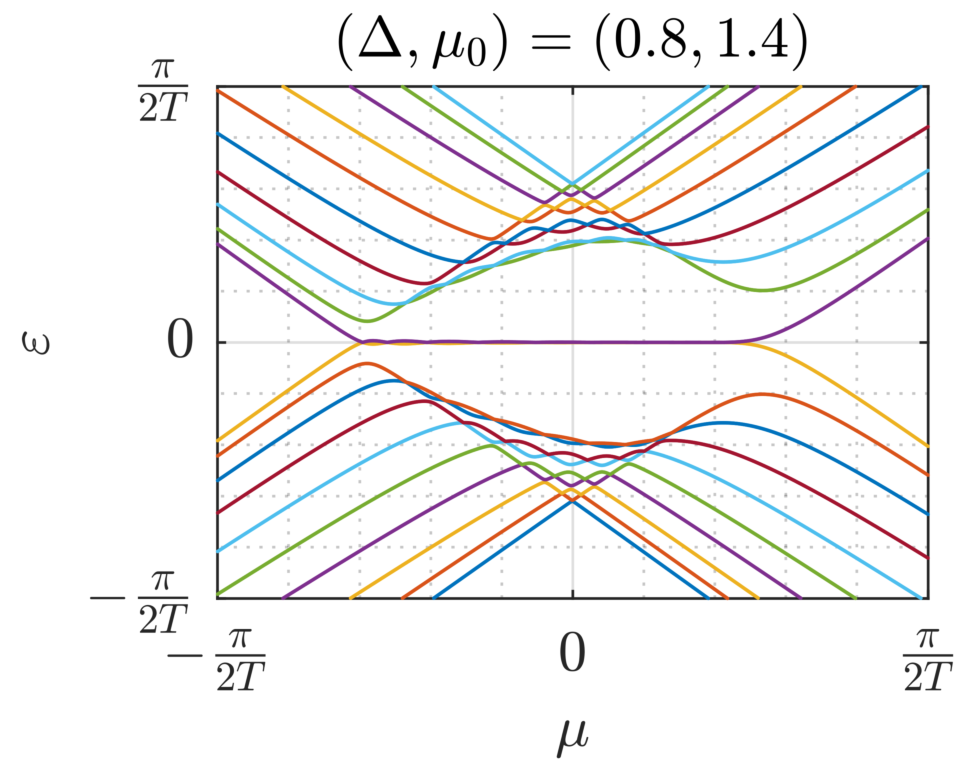
\includegraphics[scale=1]{Figures/New/Quasienergies_Exact4.png}\\
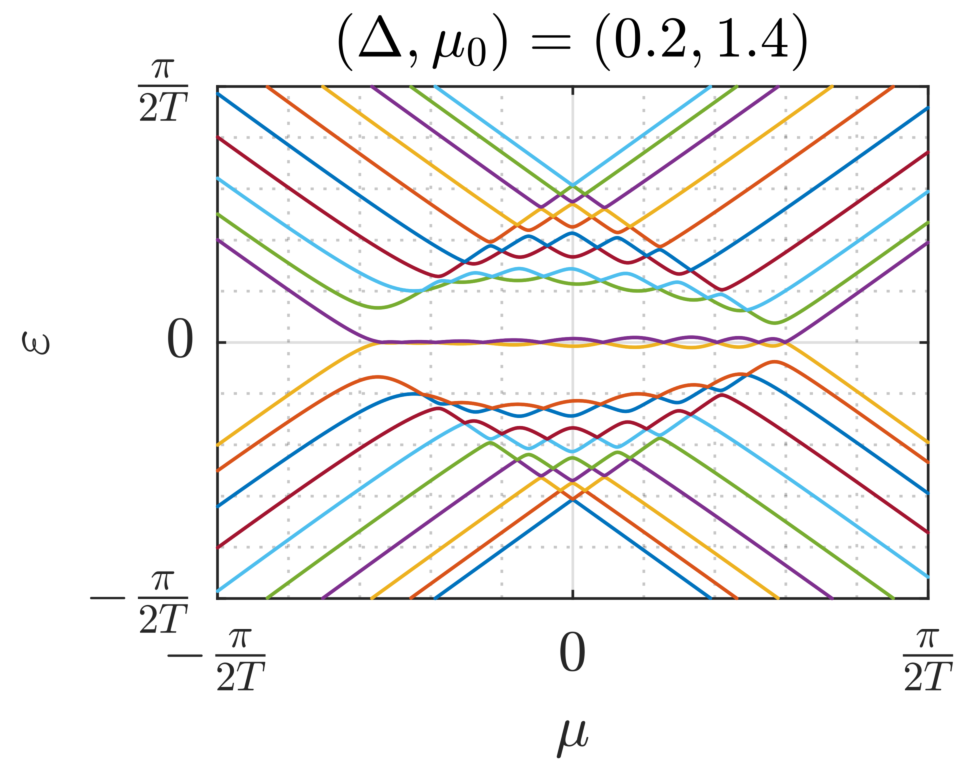
\includegraphics[scale=1]{Figures/New/Quasienergies_Expansion3.png}%
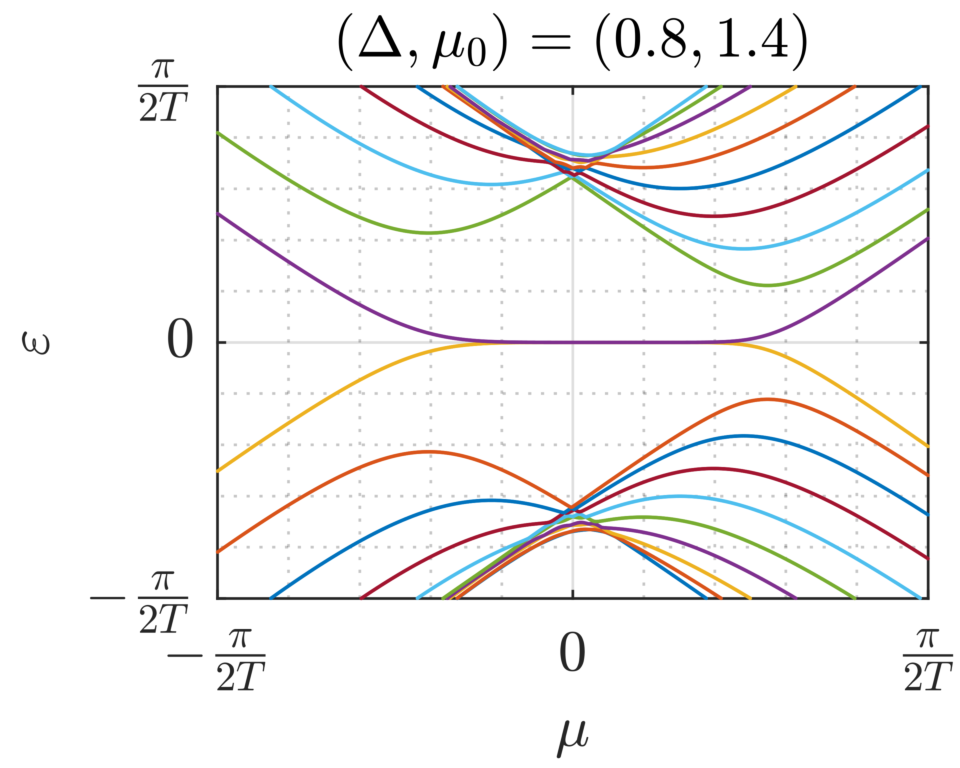
\includegraphics[scale=1]{Figures/New/Quasienergies_Expansion4.png}\\
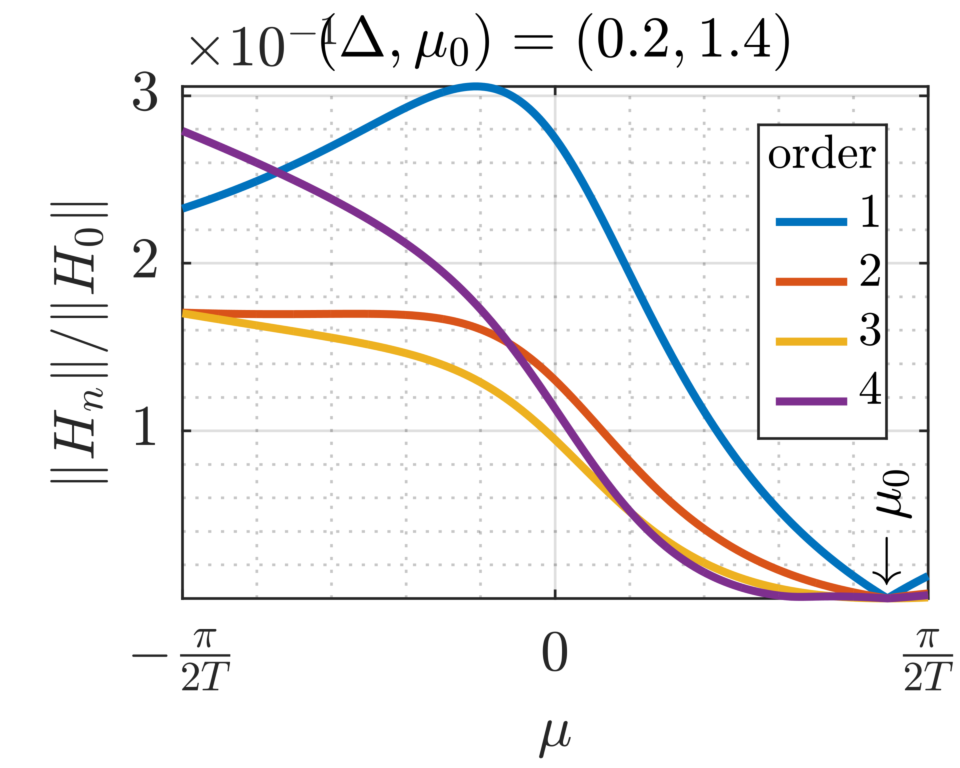
\includegraphics[scale=1]{Figures/New/Expansion_Amplitude3.png}%
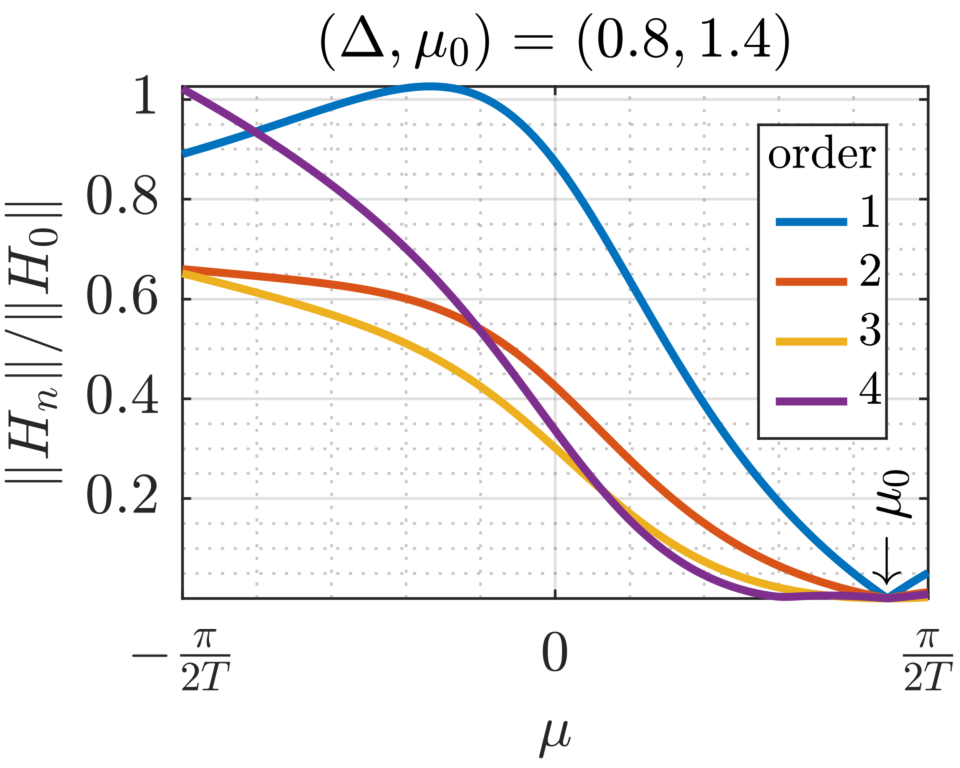
\includegraphics[scale=1]{Figures/New/Expansion_Amplitude4.png}\\
\caption{Top row: exact quasienergies. Middle row: quasienergies calculated by $2^{\text{nd}}$ order BCH approximation. Bottom row: relative norm of the four first BCH expansion terms.}
\label{Fig:5}
\end{figure}

We saw in the previous plots how the main effect of $\mu_0$ is a translation in our plots of $\en$ vs. $\mu_1$. We will remove this from now on by plotting instead $\en$ vs. $\mu = \mu_0 + \mu_1$. In the last plot of Fig.~2 we also saw that $\mu_0$ affects the oscillations asymmetrically. We could gain some insight on this using the second order term in the BCH expansion. However, we also saw that the asymmetry appears for larger values of $\Delta$ and $\mu_0$, meaning a perturbative calculation might not be correct anymore. Defining the norm of a matrix $M$ as $||M|| = \sqrt{\mathrm{Tr}( M^{\dagger}M)}$, and given $H_F = \sum_n H_F^{(n)}$ where $H_F^{(n)}$ is the term in the BCH expansion of order $n$, we show in Figs.~\ref{Fig:4}~and~\ref{Fig:5} a comparison of the quasienergies calculated exactly and using the BCH second order expansion, with the relative norm plotted in the last row of panels. For $\mu_0 = 0$ the agreement is quite good, even for higher $\Delta$, as seen clearly in the first two rows but also in the norm. When $\mu_0 = 1.4$, the disagreement is clear as we move away from $\mu = \mu_0$, and we see in the last panel that eventually higher order terms are more relevant and the perturbation approach is no longer valid. It seems that the BCH expansion approach is quite limited since it is only valid when we can approximate the quasienergies directly by the energies of the Kitaev chain. However, It is interesting that the asymmetry effect seen before in the exact quasienergies and again in Fig.~\ref{Fig:5} on the top right seems to appear on the second order calculations but for smaller values of $\Delta$ and reflected, as seen in \ref{Fig:5} center left. While the asymmetry is a feature of the system, in the second order calculation it is caused by a transition from a perturbative to a non-perturbative regime as we move away from $\mu = \mu_0$. Still, even with the disagreement in $\Delta$ and the reflection, it seems to be possible to understand something from the second order term after all. Calculating explicitly this term, we have
%
\begin{equation} 
\begin{split}
  &H_F^{(2)} = \frac{T^2}{12}( [M_0,[M_0,M_1]]+[M_1,[M_1,M_0]] ) =\\
  &\frac{T^2 \Delta \mu_1}{6} \left(\begin{matrix}
0 & - \Delta & 0 & - \mu_d & 0 & J_y \\
 \Delta & 0 & - \mu_d & 0 & J_x & 0 \\
 0 &  \mu_d & 0 & - \Delta & 0 & - \mu_d  & \dots \\ 
 \mu_d & 0 & \Delta & 0 & - \mu_d & 0 \\ 
 0 & - J_x & 0 & \mu_d & 0 & - \Delta \\ 
 - J_y & 0 & \mu_d & 0 & \Delta & 0\\ 
  & & \vdots & & & & 
  \end{matrix} \right),
\end{split}
\end{equation}
% 
where $\mu_d = \mu_0 - \mu_1 $. Labeling the matrix entries by $(i,j)$, we see that this matrix is zero when $i+j$ is even, just like the zero order term but in contrast with the term of first order in Eq.~\ref{eq:1st_order} which is zero in odd entries. It is possible to prove that all terms of even (odd) order are null in all even (odd) entries given that they are all generated by successive multiplications of $M_0$ and $M_1$ which are zero in the even entries. Let us recall now the zero order term:
%
\begin{equation}
\begin{split}
 H_F^{(0)}& = M_0+M_1 =\\
		&\left(\begin{matrix}
		0 & \mu & 0 & -J_y & 0 & 0 \\
		-\mu & 0 & J_x & 0 & 0 & 0  \\
		0 & -J_x & 0 & \mu & 0 & -J_y & \dots \\
		J_y & 0 & -\mu & 0 & J_x & 0 \\
		0 & 0 & 0 & -J_x & 0 & \mu \\
		0 & 0 & J_y & 0 & -\mu & 0\\
		 & & \vdots & & & 
	\end{matrix} \right).
\end{split}
\end{equation}	
%
We see the overlap in non-zero entries of both matrices, while $H_F^{(2)}$ has two extras entries of values $J_x$ and $J_y$. Let us ignore these two terms and call this new matrix $\bar{H}_F^{(2)}$. Then, $\bar{H}_F = H_F^{(0)} + \bar{H}_F^{(2)}$ corresponds to a static Kitaev model with new effective parameters\footnote{We also ignore the first order term since it has no entries that overlap the zero order.}:
%
\begin{align}
t\eff &= t, \\
\Delta\eff &= \Delta - \frac{T^2 \Delta \mu_1 \mu_d}{3}, \\
\mu\eff &= \mu - \frac{T^2 \Delta^2 \mu_1}{6}
\end{align}
%
We know these expressions won't be valid in any interesting regime of parameters, but at least they agree qualitatively with several things. In the static topological phase, we only have crossings when $| \Delta | < 1$ and a smaller $| \Delta |$ reduces the gap and increases the oscillation amplitude. We saw previously how there are zero energy Majoranas which cross even for high $\Delta$ or even outside the static topological phase. but now the parameters are mapped into new parameters which can fall into a different phase

Correcting the reflection is simple, we just have to change the sign of $\mu_0$, so we have $\mu_d \rightarrow -\mu$.


\subsection*{Edge spin (Majorana) autocorrelator}
(to be expanded...)
%As for possible physical consequences, I'll only point out that due to the crossings we have exact zero quasienergies which should have long time consequences since $U(nT) = U(T)^n$. 

\bibliographystyle{plain}
\bibliography{bib}

\end{document}
